\chapter{Zanarkand}
\restartlist{enumerate}
\begin{enumerate}
	\liteversiondetermination{Exclude}{%
		\item walk left. \fmv+\cs[2:20]
		\item Move left to the sphere, \sd, \cs[1:40]. Walk further left and follow the path down, \cs[3:20], walk left onto the next screen.
	}
	\item Charge \tidus, \rikku\ and \lulu\ \od. Best Encounters are Behemoth on broken bridge and Defender Z inside the dome.
	\item Also Charge \yuna\ \od\ if not already done.
\end{enumerate}
\begin{enumerate}[resume]
	\liteversiondetermination{Exclude}{\item Continue on the path and into the dome.}
	\item Before Spectral Keeper:
	\begin{itemize}
		\item \formation{\rikku}{\lulu}{\auron}
		\item Heal everyone except \rikku. \important{Rikku must remain in critical HP for the Spectral Keeper fight.}% using the \rikku command raises an error
	\end{itemize}
\end{enumerate}
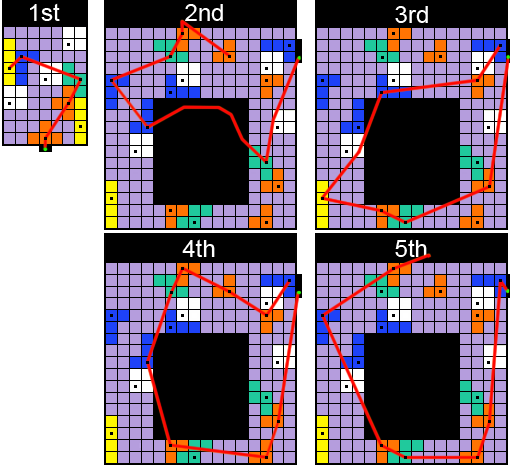
\includegraphics[width=.95\columnwidth]{graphics/Zanarkand_Trials}
\liteversiondetermination{Exclude}{%
\begin{enumerate}[resume]
	\item Push in the pedestals starting from the Top Left, to Bottom Left, then Top Right, Bottom Right, then Besaid Sphere. After pushing in each pedestal, do the corresponding puzzle, shown above.
	\item After the second puzzle, take the Kilika Sphere on the left and put it into the second pedestal.
	\item After the fifth puzzle, take the Besaid Sphere from the right and put it into the fifth pedestal.
	\item \cs, run into the large room
\end{enumerate}
}
\begin{battle}[52000]{Spectral Keeper}
	\begin{itemize}
		\rikkuf Use Light Curtain on \auron
		\auronf Defend
		\luluf Switch Weapon
		\rikkuf Mix 2x Wings to Discovery
		\luluf Thunder Fury (Exactly 5 hits)
		\enemyf Attack All
		\enemyf Berserk Tail
		\auronf Attack
	\end{itemize}
\end{battle}
\begin{enumerate}[resume]
	\item Switch \auron\ for \tidus
	\item If \lulu\ didn't get hit by Spectral Keeper run back out of the Trials and force encounters to charge her \od
	\item Heal everyone except \rikku\ before Yunalesca. \important{Rikku must remain in critical HP for the Yunalesca fight.}% using the \rikku command raises an error
	\liteversiondetermination{Exclude}{\item Run up, \sd\ by mashing another button (like \textbf{R1}) at the same time as confirm, walk up to Yunalesca's room, \sd}
\end{enumerate}
\begin{battle}[132000]{Yunalesca}
	\begin{itemize}
		\rikkuf Light Curtain on Self
		\tidusf Switch Weapon
		\luluf Switch Weapon
		\rikkuf Mix 2x Wings to Discovery
		\switch{\tidus}{\wakka}, Defend
		\switch{\lulu}{\auron}, Hi-Potion \rikku
		\enemyf Dispelling Slap
		\enemyf Absorb
		\wakkaf Hi-Potion \rikku\ if she is damaged, otherwise defend
		\rikkuf Use Fire Gem
		\switch{\auron}{\tidus}, Slice and Dice
		\switch{anyone}{\lulu}, Thunder Fury (7 hits required)
	\end{itemize}
\vspace{\baselineskip}
Check what equipment drops from Yunalesca. Any weapon dropped by Yunalesca will have \textbf{Zombiestrike} which will be important for later.
\end{battle}
\liteversiondetermination{Exclude}{%
\begin{enumerate}[resume]
	\item \sd, leave room, walk down steps, \sd, go down on the next screens, \save, go up the lift, walk out of the cloister of trials, walk down the steps, walk down, \sd\ during \cs+\skippablefmv
\end{enumerate}
}